\documentclass[12pt,a4paper]{article}

%\usepackage[left=1.5cm,right=1.5cm,top=1cm,bottom=2cm]{geometry}
\usepackage[in, plain]{fullpage}
\usepackage{array}
\usepackage{../../../pas-math}
\usepackage{../../../moncours}


%\usepackage{pas-cours}
%-------------------------------------------------------------------------------
%          -Packages nécessaires pour écrire en Français et en UTF8-
%-------------------------------------------------------------------------------
\usepackage[utf8]{inputenc}
\usepackage[frenchb]{babel}
\usepackage[T1]{fontenc}
\usepackage{lmodern}
\usepackage{textcomp}



%-------------------------------------------------------------------------------

%-------------------------------------------------------------------------------
%                          -Outils de mise en forme-
%-------------------------------------------------------------------------------
\usepackage{hyperref}
\hypersetup{pdfstartview=XYZ}
%\usepackage{enumerate}
\usepackage{graphicx}
\usepackage{multicol}
\usepackage{tabularx}
\usepackage{multirow}


\usepackage{anysize} %%pour pouvoir mettre les marges qu'on veut
%\marginsize{2.5cm}{2.5cm}{2.5cm}{2.5cm}

\usepackage{indentfirst} %%pour que les premier paragraphes soient aussi indentés
\usepackage{verbatim}
\usepackage{enumitem}
\usepackage[usenames,dvipsnames,svgnames,table]{xcolor}

\usepackage{variations}

%-------------------------------------------------------------------------------


%-------------------------------------------------------------------------------
%                  -Nécessaires pour écrire des mathématiques-
%-------------------------------------------------------------------------------
\usepackage{amsfonts}
\usepackage{amssymb}
\usepackage{amsmath}
\usepackage{amsthm}
\usepackage{tikz}
\usepackage{xlop}
%-------------------------------------------------------------------------------



%-------------------------------------------------------------------------------


%-------------------------------------------------------------------------------
%                    - Mise en forme avancée
%-------------------------------------------------------------------------------

\usepackage{ifthen}
\usepackage{ifmtarg}


\newcommand{\ifTrue}[2]{\ifthenelse{\equal{#1}{true}}{#2}{$\qquad \qquad$}}

%-------------------------------------------------------------------------------

%-------------------------------------------------------------------------------
%                     -Mise en forme d'exercices-
%-------------------------------------------------------------------------------
%\newtheoremstyle{exostyle}
%{\topsep}% espace avant
%{\topsep}% espace apres
%{}% Police utilisee par le style de thm
%{}% Indentation (vide = aucune, \parindent = indentation paragraphe)
%{\bfseries}% Police du titre de thm
%{.}% Signe de ponctuation apres le titre du thm
%{ }% Espace apres le titre du thm (\newline = linebreak)
%{\thmname{#1}\thmnumber{ #2}\thmnote{. \normalfont{\textit{#3}}}}% composants du titre du thm : \thmname = nom du thm, \thmnumber = numéro du thm, \thmnote = sous-titre du thm

%\theoremstyle{exostyle}
%\newtheorem{exercice}{Exercice}
%
%\newenvironment{questions}{
%\begin{enumerate}[\hspace{12pt}\bfseries\itshape a.]}{\end{enumerate}
%} %mettre un 1 à la place du a si on veut des numéros au lieu de lettres pour les questions 
%-------------------------------------------------------------------------------

%-------------------------------------------------------------------------------
%                    - Mise en forme de tableaux -
%-------------------------------------------------------------------------------

\renewcommand{\arraystretch}{1.7}

\setlength{\tabcolsep}{1.2cm}

%-------------------------------------------------------------------------------



%-------------------------------------------------------------------------------
%                    - Racourcis d'écriture -
%-------------------------------------------------------------------------------

% Angles orientés (couples de vecteurs)
\newcommand{\aopp}[2]{(\vec{#1}, \vec{#2})} %Les deuc vecteurs sont positifs
\newcommand{\aopn}[2]{(\vec{#1}, -\vec{#2})} %Le second vecteur est négatif
\newcommand{\aonp}[2]{(-\vec{#1}, \vec{#2})} %Le premier vecteur est négatif
\newcommand{\aonn}[2]{(-\vec{#1}, -\vec{#2})} %Les deux vecteurs sont négatifs

%Ensembles mathématiques
\newcommand{\naturels}{\mathbb{N}} %Nombres naturels
\newcommand{\relatifs}{\mathbb{Z}} %Nombres relatifs
\newcommand{\rationnels}{\mathbb{Q}} %Nombres rationnels
\newcommand{\reels}{\mathbb{R}} %Nombres réels
\newcommand{\complexes}{\mathbb{C}} %Nombres complexes


%Intégration des parenthèses aux cosinus
\newcommand{\cosP}[1]{\cos\left(#1\right)}
\newcommand{\sinP}[1]{\sin\left(#1\right)}


%Probas stats
\newcommand{\stat}{statistique}
\newcommand{\stats}{statistiques}
%-------------------------------------------------------------------------------

%-------------------------------------------------------------------------------
%                    - Mise en page -
%-------------------------------------------------------------------------------

\newcommand{\twoCol}[1]{\begin{multicols}{2}#1\end{multicols}}


\setenumerate[1]{font=\bfseries,label=\textit{\alph*})}
\setenumerate[2]{font=\bfseries,label=\arabic*)}


%-------------------------------------------------------------------------------
%                    - Elements cours -
%-------------------------------------------------------------------------------





%\makeatletter
%\renewcommand*{\@seccntformat}[1]{\csname the#1\endcsname\hspace{0.1cm}}
%\makeatother


%\author{Olivier FINOT}
\date{}
\title{Information chiffrée }

%\newcommand{\disp}{false}

\lhead{CH2 : Suites numériques}
\rhead{O. FINOT}
%
%\rfoot{Page \thepage}
\begin{document}
%\maketitle

\chap[num=3, color=red]{Séries statistiques à deux variables}{Olivier FINOT, \today }

\begin{myobj}
	\begin{itemize}
		
		\item Construire le symétrique d’un point ou d'une figure par rapport à une droite à la main où à l’aide d’un logiciel;
		\item Construire le symétrique d’un point ou d'une figure par rapport à un point, à la main où à l’aide d’un logiciel;
		\item Utiliser les propriétés de la symétrie axiale ou centrale;
		\item Identifier des symétries dans des figures.		
	\end{itemize}
\end{myobj}

\begin{mycomp}
	\begin{itemize}
		\item \kw{Chercher (Ch2)} :  s’engager    dans    une    démarche    scientifique, observer, questionner, manipuler, expérimenter (sur une feuille de papier, avec des objets, à l’aide de logiciels), émettre des hypothèses, chercher des exemples ou des contre-exemples, simplifier ou particulariser une situation, émettre une conjecture ;
		\item \kw{Raisonner (Ra3)} :  démontrer : utiliser un raisonnement logique et des règles établies (propriétés, théorèmes, formules) pour parvenir à une conclusion ;
		\item \kw{Communiquer (Co2)} :  expliquer à l’oral ou à l’écrit (sa démarche, son raisonnement, un calcul, un protocole   de   construction   géométrique, un algorithme), comprendre les explications d’un autre et argumenter dans l’échange ; 
		
	\end{itemize}
\end{mycomp}




\section{Statistiques à une variable (révisions)}

\subsection{Médiane et moyenne}
\begin{mydef}
	La \kw{médiane $Me$} d'une série statistique est le nombre qui \kw{partage la série en deux} séries ayant \kw{le même effectif}.
	
	La moitié (ou 50 \%)  des valeurs de la série sont inférieures ou égales à la médiane et l'autre moitié (50 \%) lui sont supérieures ou égales.
\end{mydef}

\begin{mydef}
	On note $x_1, x_2, ..., x_p$ les valeurs du caractère étudié et $n_1, n_2, ...,n_p$ les effectifs correspondants.
	
	La \kw{moyenne $\bar{x}$} de la série statistique est $\bar{x} = \dfrac{n_1x_1 + n_2x_2 + ... + n_px_p}{N} = \dfrac{\Sigma n_ix_i}{N} $
	
\end{mydef}

\subsection{\'Etendue}

\begin{mydef}
	L'\kw{étendue $e$} d'une série statistique est la différence entre la plus grande et la plus petite valeur de la série.
\end{mydef}	



\subsection{Quartiles}

\begin{mydef}
	\begin{itemize}
		\item Le \kw{premier quartile $Q_1$}, est la plus petite valeur à laquelle un quart (ou 25 \%) des valeurs sont inférieures ou égales.
		\item Le \kw{troisième quartile $Q_3$}, est la plus petite valeur à laquelle trois quarts (ou 75 \%) des valeurs sont inférieures ou égales.
		\item L'\kw{écart interquartile $Q_3-Q_1$} est la différence entre les 3$^e$ et 1$^{er}$ quartiles : $Q_3 - Q_1$. Il regroupe au moins 50 \% des effectifs de la série avec un nombre égal de valeurs réparties de part et d'autre de la médiane $Me$.
	\end{itemize}
	
\end{mydef}	

\subsection{\'Ecart type}

\begin{mydef}
	L'\kw{écart type $\sigma$} (sigma), fourni par la calculatrice ou le tableur, mesure la dispersion de la série autour de la moyenne $\bar{x}$. 
	
	Plus l'écart type $\sigma$ est grand, plus les valeurs sont <<\kw{dispersées}>> autour de la moyenne. 
	
	Inversement, plus l'écart type $\sigma$ est grand, plus les valeurs sont <<\kw{resserrées}>> autour de la moyenne.
\end{mydef}	

\section{Tableaux croisés d'effectifs}


\subsection{Rappel sur les fréquences}

\begin{mydef}
	La fréquance $f$ d'une population $A$ dans une population $E$ est le rapport des effectifs :
	
	\begin{eqnarray*}
		f & = & \dfrac{n_A \; (Effectif de A) }{n_E \; (Effectif de E)}  \\
	\end{eqnarray*}
\end{mydef}


\begin{myex}
	On considère les montant des achats, en euros de $N = 200$ personnes dans une pharmacie un jour donné :
	
	\begin{center}
		
		\begin{tabular}{|@{\ }l@{\ }|@{\ }c@{\ }|@{\ }c@{\ }|@{\ }c@{\ }|@{\ }c@{\ }|}
			\hline
			Montant des achats & {[}0, 20{[} & {[}20, 40{[} & {[}40, 60{[} & {[}60, 80{[} \\ \hline
			Effectif $n_i$      & 52          & 110          & 30           & 8            \\ \hline
			Fréquence $f_i$     & \num{0.26}        & \num{0.55}         & \num{0.15}         & \num{0.04}         \\ \hline
		\end{tabular}
	\end{center}	
\end{myex}

\subsection{Fréquence conditionnelle}

\begin{myact}{La suite des nombres impairs}
	On considère la suite des nombres impairs, 1, 3, 5, 7, ..., que l'on note successivement $u_1$, $u_2$, $u_3$, $u_4$...
	Donc $u_1=1$, $u_2=3$, $u_3=5$...\\
	
	\begin{enumerate}[label=\arabic*)]
		\item \begin{enumerate}[label=\alph*.]
			\item Compléter : $u_4=.....$, $u_? =15$, $u_{10}=......$.
			\item Quel est le premier terme de la suite ?
			\item Comment passe-t-on d'un terme au suivant ?
			\item $n$ est est nombre entier positif non nul, on s'intéresse au terme de rang $n$ (donc le $n^{ième}$ nombre impair). Exprimer $u_{n+1}$ en fonction de $u_n$.
			\item Exprimer $u_n$ en fonction de $n$.
			\item Calculer $u_{100}$, $u_{150}$, $u_{1000}$.
		\end{enumerate} 
		
		\item Somme de nombres impairs. 
		
		On note $S_1=u_1=1$; $S_2=u_1+u_2=1+3=4$; puis, plus généralement $S_n=u_1+u_2+u_3+...+u_n$.
		
		\begin{enumerate}
			\item Compléter le tableau suivant :\\
			\begin{tabular}{|@{\ \ }l@{\ \ }|@{\ \ }c@{\ \ }|@{\ \ }c@{\ \ }|@{\ \ }c@{\ \ }|@{\ \ }c@{\ \ }|@{\ \ }c@{\ \ }|@{\ \ }c@{\ \ }|@{\ \ }c@{\ \ }|@{\ \ }c@{\ \ }|}
				\hline
				$n$   & 1 & 2 & 3 & 4 & 5 & 6 & 7 & 8 \\ \hline
				$u_n$ & 1 & 3 & 5 &   &   &   &   &   \\ \hline
				$S_n$ & 1 & 4 &   &   &   &   &   &   \\ \hline
			\end{tabular}
			
			\item En déduire une relation entre $S_{n+1}$, $S_{n}$, et $u_{n+1}$.
			
			\item En observant les résultats du tableau conjecturer une expression de $S_n$ en fonction de $n$.
		\end{enumerate}
	\end{enumerate}
	
	
\end{myact}

\begin{enumerate}[label=\arabic*)]
	\item \begin{tabular}{|@{\ }l@{\ }|@{\ }c@{\ }|@{\ }c@{\ }|@{$\quad$}c@{$\quad$}|}
		\hline
		& Compétition $(C)$ & Pas compétition $(\bar{C})$ & Total \\ \hline
		Fumeurs  $(F)$   & 18 & 36 & 54 \\ \hline
		Non fumeurs $(\bar{F})$ & 216 & 90 & 306 \\ \hline
		Total & 234 & 126 & 360 \\ \hline
	\end{tabular}

	\item \begin{enumerate}[label=\alph*)]
		\item \begin{eqnarray*}
			f(C) &=& \frac{Effectif\; de\; C}{Effectif\; total} \\
			f(C) &=& \frac{234}{360} \\
			f(C) &=& \num{0.65}
		\end{eqnarray*}
	
	La proportion de personnes pratiquant la compétition est \num{0.65}.
	
		\item \begin{eqnarray*}
			f(F) &=& \frac{Effectif\; de\; F}{Effectif\; total} \\
			f(F) &=& \frac{54}{360} \\
			f(F) &=& \num{0.15}
		\end{eqnarray*}
		
		La proportion de fumeurs est \num{0.15}.
		
		\item \begin{eqnarray*}
			f(F \cap C) &=& \frac{Effectif\; des\; fumeurs \; pratiquant\; la\; compétition}{Effectif\; total} \\
			f(F \cap C) &=& \frac{18}{360} \\
			f(F \cap C) &=& \num{0.05}
		\end{eqnarray*}
		
		La proportion de personnes qui fument et pratiquent la compétition est \num{0.05}.
		
		\item \begin{eqnarray*}
			f_C(F) &=& \frac{Effectif\; des\; fumeurs \; pratiquant\; la\; compétition}{Effectif\; des\; personnes\; pratiquant\; la\; compétition} \\
			f_C(F) &=& \frac{18}{234} \\
			f_C(F) &\approx& \num{0.08}
		\end{eqnarray*}
		
		La proportion de fumeurs parmi les personnes pratiquent la compétition est \num{0.08}.
		
		\item \begin{eqnarray*}
			f(F \cup C) &=& \frac{fumeurs + pratiquants - fumeurs\; pratiquants}{Effectif\; total} \\
			f(F \cup C) &=& \frac{54 + 234 - 18}{360} \\
			f(F \cup C) &=& \frac{270}{360} \\
			f(F \cup C) &=& \num{0.75}
		\end{eqnarray*}
		
		La proportion de personnes qui fument ou pratiquent la compétition est \num{0.75}.
	\end{enumerate}

\end{enumerate}


\begin{mybilan}
	$A$ et $B$ sont deux sous-populations d'une population $E$.
	\begin{itemize}
		\item $\mathbf{f(B)}$ est la \kw{fréquence marginale} de $B$ :
		
		\begin{eqnarray*}
			f(B) &=& \dfrac{Effectif\; de\; B }{Effectif\; de\; E}
		\end{eqnarray*}
	
		\item $\mathbf{f(A \cap B)}$ est la \kw{fréquence conjointe} de $A$ et $B$ :
		
		\begin{eqnarray*}
			f(A \cap B) &=& \dfrac{Effectif\; du\; croisement \; de\;A\; et\; de\; B }{Effectif\; de\; E}
		\end{eqnarray*}
	
		\item $\mathbf{f(A \cup B)}$ est la \kw{fréquence de la réunion} de $A$ et $B$ :
		
		\begin{eqnarray*}
			f(A \cup B) &=& \dfrac{Eff.\; de\; A + Eff.\; de\; B  - Eff.\; du\; croisement \; de\;A\; et\; de\; B}{Effectif\; de\; E}
		\end{eqnarray*}
	
		\centering{ou}
		\begin{eqnarray*}
			f(A \cup B) &=& f(A) + f(B) - f(A \cap B)
		\end{eqnarray*}
	
		\item $\mathbf{f_B(A)}$ est la \kw{fréquence conditionnelle} de $A$ \kw{sachant} $B$ :
		
		\begin{eqnarray*}
			f_B(A) &=& \dfrac{Effectif\; du\; croisement \; de\;A\; et\; de\; B }{Effectif\; de\; B}
		\end{eqnarray*}
	
		\centering{ou} 				
		\begin{eqnarray*}
			f_B(A) &=& \dfrac{f(A \cap B)}{f(B)}
		\end{eqnarray*}
	
	
	\end{itemize}
\end{mybilan}

\newpage

\section{Statistiques à deux variables}

\subsection{Définition et représentation graphique}

\begin{mybilan}
	\begin{itemize}
		\item Lorsqu'on étudie \kw{deux caractères statistiques} sur une même population, on obtient une \kw{série statistique double}.
		
		\item La représentation d'une série statistique double forme un \kw{nuage de points}.
		
		\item Le \kw{point moyen} $G$ d'un  nuage de points a pour coordonnées \kw{$(\bar{x}; \bar{y})$}.
	\end{itemize}
	

\end{mybilan}

	\begin{myexs}
	\begin{enumerate}
		\item 	Soit ($u_n$) la suite arithmétique de terme initial $u_0 = 1,5$ et de raison $r = -7$.
		
		Le terme de rang $n$ est $u_n = 1,5 + n \times (-7)$ c'est à dire $u_n=1,5 - 7n$.
		
		On a ainsi : 
		\begin{itemize}
			\item $u_4 = 1,5 - 7 \times 4 = -26,5$
			\item $u_{100} = 1,5 - 7 \times 100 = -698,5$
		\end{itemize}
		
		\item Soit ($u_n$) la suite arithmétique de terme initial $u_1 = 14$ et de raison $r = 1,3$.
		
		Le terme de rang $n$ est $u_n = 14 + (n-1) \times 1,3$; c'est à dire $u_n = 12,7 + 1,3n$.

		On a ainsi : 
		\begin{itemize}
			\item $u_4 = 12,7 + 1,3 \times 4 = 17,9$;
			\item $u_{100} = 12,7 + 1,3 \times 100 = 142,7$.
		\end{itemize}
	\end{enumerate}

	
	
\end{myexs}
	
	
\subsection{Ajustement affine}

\begin{mybilan}
	\begin{itemize}
		\item Si le nuage de points a une forme <<allongée>>, on peut calculer un \kw{ajustement affine} du nuage. 
		\item On obtient ainsi une \kw{droite d'ajustement} (ou droite de régression) qui passe par le point moyen $G$ et au plus près des autres points du nuage.		
	\end{itemize}
\end{mybilan}


\begin{myex}
	La droite d'ajustement obtenue grâce au tableur passe par le point moyen $G$ dont nous avons calculé les coordonnées.
	\begin{center}
		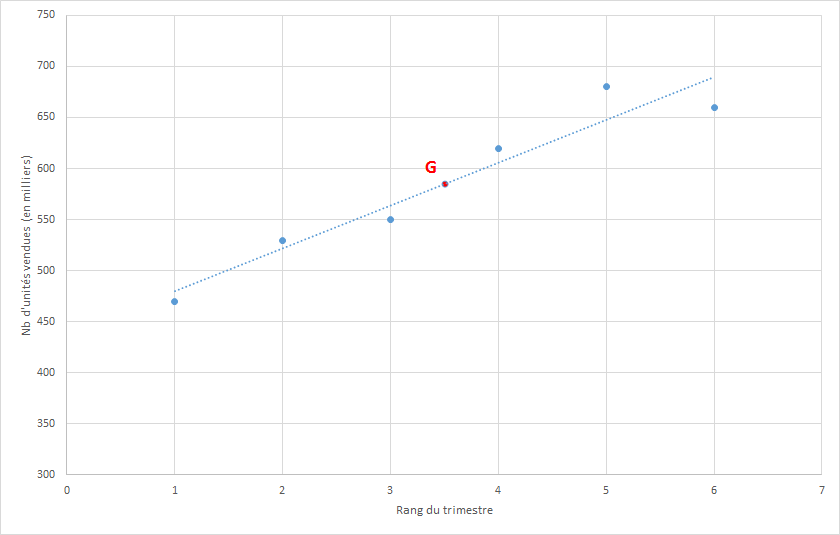
\includegraphics[scale =0.7]{./img/graph2}		
	\end{center}

\end{myex}


\subsection{Prévisions}

\begin{mymeth}
	\begin{itemize}
		\item La droite d'ajustement donne la <<tendance>> de l'évolution de la grandeur $y$ en fonction de celle de $x$.
		\item En supposant que la tendance se poursuive, il est possible d'estimer une valeur future par lecture graphique ou à partir de l'équation de la droite. 
	\end{itemize}
	
	
	%L'équation de type $y = ax +b $ de la droite d'ajustement donne  Cette équation permet de réaliser des estimations en supposant que la tendance observée se poursuive.
\end{mymeth}

\begin{myex}
	Ici on considère la répartition des prix du gazole dans l'ensemble des 25 stations du département :
	
	\begin{center}
		\begin{tabular}{|@{\ }l@{\ } | @{\ }c@{\ } | @{\ }c@{\ } | @{\ }c@{\ } |@{\ }c@{\ } |@{\ }c@{\ } |@{\ }c@{\ }|@{\ }c@{\ }|@{\ }c@{\ }|@{\ }c@{\ }|@{\ }c@{\ }|}
			\hline
			Prix & 1,368 & 1,369 & 1,374 & 1,375 & \kw{1,377} & \kw{1,379} & 1,385 & 1,408 & 1,450 & 1,460 \\ \hline			
			Nb. de stations & 2 & 5 & 2 & 4 & 1 & 4 & 2 & 1 & 3 & 1 \\ \hline
		\end{tabular}
	\end{center}
	
	\kw{Moyenne} des prix des 25 stations : 
	\begin{center}
		$\bar{x} = \dfrac{1,368 \times 2 + 1,369 \times 5 + ... + 1,450 \times 3 + 1,460}{25} = 1,3884$
	\end{center}
	
	Le prix moyen observé pour ces 25 stations est 1,3884 €.	 
	
\end{myex}

\end{document}